\chapter{Verwandte Arbeiten}
\label{chap:related_work}

In diesem Kapitel werden zu dieser Arbeit relevante ähnliche Arbeiten,
die durch ein technisches Identifikationsmittel Produkte finden und
mit Informationen dazu anzeigen können, verglichen.

Die Arbeit soll dabei jeweils einen Bezug zur Veganität von einem
Produkt aufweisen und dies auch mit Quellen belegen können.
Zudem soll die Arbeit eine mobile Anwendung bereitstellen, damit auch
z.\,B. im Supermarkt nach einem Produkt gesucht werden kann.
Des weiteren sollen die Produktdaten in der jeweiligen Arbeit
lizenzfrei erhältlich sein, d.\,h. die Daten können entweder per
\ac{API}, also einer Programmierschnittstelle, oder als kompletter
Speicherauszug aus der Datenbank bezogen werden.
Auch der Zugang zu der Website oder der mobilen App selbst soll ohne
Anmeldung
und kostenlos möglich sein.
Zudem sollen die Produktdaten von den Nutzer*innen stammen, indem
diese die Daten beispielsweise wie in einem Wiki eintragen können.
Zuletzt soll die Arbeit mehrsprachig verfügbar sein, um so auch in
anderen Ländern genutzt werden zu können.

Im Folgenden werden vier Arbeiten
vorgestellt, die bei diesem Werk von Relevanz sind: zwei
kommerzielle Websites (barcoo und das-ist-drin), eine Diplomarbeit
(\acs{EuLaA}) und ein Forschungsprojekt 
(\acs{MENSSANA}).
Eine Zusammenfassung und damit die Herausstellung der einzelnen
Kriterien erfolgt am Schluss des Kapitels (siehe \ref{rel:zsf}).

\section{barcoo}
\label{sec:related:barcoo}

barcoo bezeichnet sich selbst als der größte Produkt-Guide in Europa
und wird von dem Unternehmen "`checkitmobile GmbH"'
entwickelt \citeweb{barcoo:about}.\\
barcoo bündelt dabei eigene Daten (die
u.\,a. von Benutzer*innen
stammen) und fremde Daten (wie z.\,B. von "`mynetfair"' und
"`ecoinform"' \citeweb{mynetfair, ecoinform})
u.\,a. zusammen mit Preisvergleichen, Testberichten, Standorten,
Lebensmittelampeln, ökologischen Informationen, Rezepten, usw. und
stellt diese Informationen auf einen Blick dar, wobei als Beispiel in
Abbildung~\ref{img:barcoo-2} Preisvergleiche und Bewertungen zu sehen
sind \citeweb{barcoo:sources}.\\
Mobile Apps werden für die Betriebssysteme iOS, Android,
Windows Phone, bada und BlackBerry OS angeboten
\citeweb{barcoo:app}.\\
Nutzer*innen von barcoo können Produkte (ohne vorherige Anmeldung)
bewerten, kommentieren und bei
eingeschalteter Abfrage des Standorts Preise eintragen. Die
Möglichkeit Produkte selbst einzutragen gibt es allerdings nicht.\\
Vegane Produkte werden als solche gekennzeichnet, allerdings nur, wenn
sie in der veganen Produktdatenbank von "`Rezeptefuchs"', ein Portal für
Veganer*innen, vorhanden sind \citeweb{rezeptefuchs, barcoo:vegan}.\\
Das Unternehmen hinter barcoo, welches sich u.\,a. durch Werbung
finanziert, bietet einen \ac{API}-Zugang an,
allerdings nur für eingetragene Firmen mit statischer IP-Adresse
\citeweb{barcoo:api}.

\begin{figure}[ht]
	\centering
	\begin{subfigure}[b]{0.45\textwidth}
		\frame{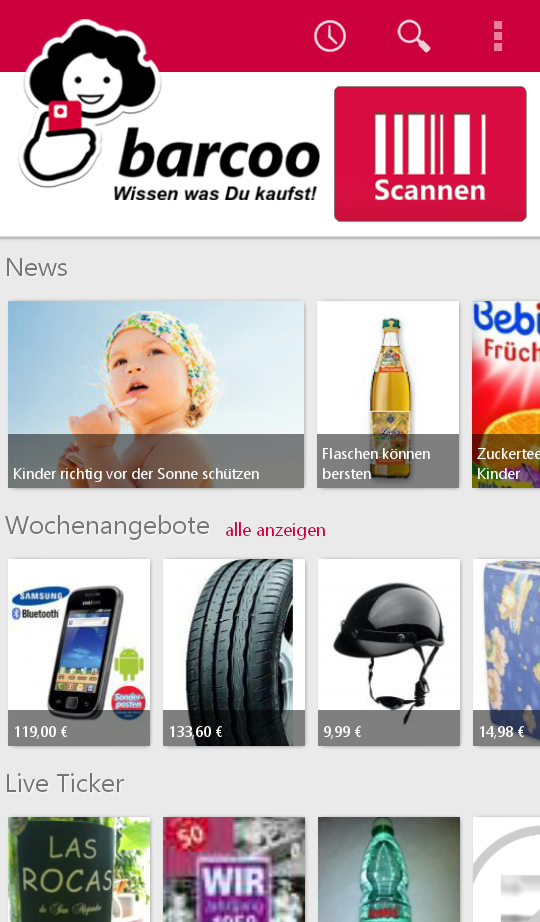
\includegraphics[width=\textwidth]{pics/barcoo-1.png}}
		\caption{direkt nach Start der App -- ein Button fordert zum Scannen auf}
		\label{img:barcoo-1}
	\end{subfigure}
	~
	\begin{subfigure}[b]{0.45\textwidth}
		\frame{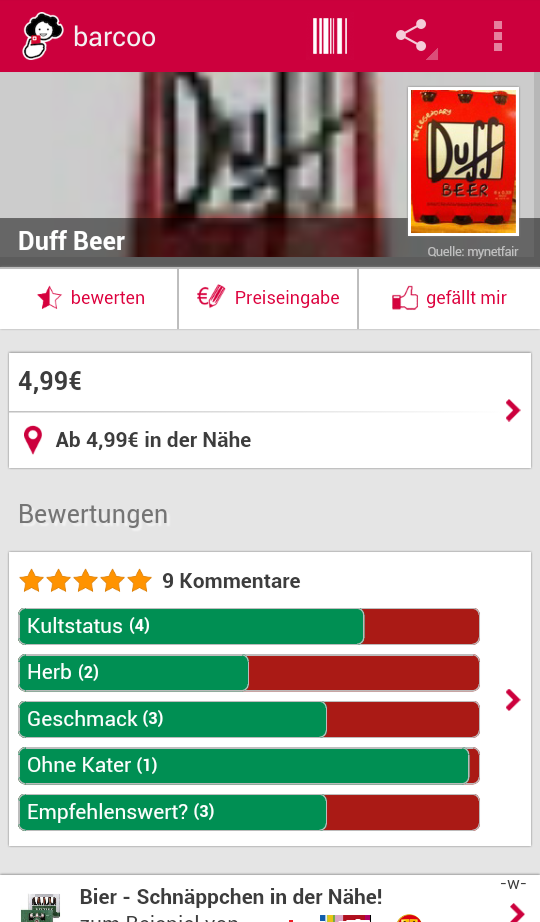
\includegraphics[width=\textwidth]{pics/barcoo-2.png}}
		\caption{Ansicht nach Scan eines Barcodes -- ein Bild,
		Preisvergleiche und Bewertungen bieten Informationen zur
Kaufentscheidung}
		\label{img:barcoo-2}
	\end{subfigure}
	\caption[Mobile barcoo-App für Android in Benutzung]{Mobile barcoo-App für Android in
	Benutzung \citeweb{barcoo:app}, aufgenommen am 16.08.2013}
	\label{img:barcoo}
\end{figure}

\section{das-ist-drin}
\label{sec:did}

\ac{DID} ist laut eigener Aussage ein Online-Verbraucherportal
der Firma "`snoopmedia GmbH"' rund um Inhalts- und Zusatzstoffe
(E-Nummern) von Lebensmitteln \citeweb{did:hilfe}.\\
\ac{DID} funktioniert nach dem Wikiprinzip, d.\,h. die Nutzer*innen können
die Produkte selbst eintragen oder ändern
(nach einer Registrierung). Es besteht auch die Möglichkeit,
dass Hersteller*innen ihre Produkte selbst verwalten.\\
\ac{DID} besitzt einen E-Nummern-Check, eine Siegeldatenbank, enthält
Informationen über Allergien oder Lebensmittelunverträglichkeiten
(bisher über 12 der 14 Haupt-Allergene) und eine
Betriebsnummernübersicht \citeweb{did:did}.\\
\ac{DID} bietet zwei mobile Varianten an: "`das-ist-drin mobil"' für
Androidgeräte, welche in Abbildung~\ref{img:did} zu sehen ist
und "`Foodtracker"', die z.\,B. Informationen darüber,
wo ein Produkt hergestellt wurde enthält, es aber nur für iOS-Geräte gibt
und daher hier nicht weiter betrachtet wird \citeweb{did:app}.

\begin{figure}[ht]
	\centering
	\begin{subfigure}[b]{0.45\textwidth}
		\frame{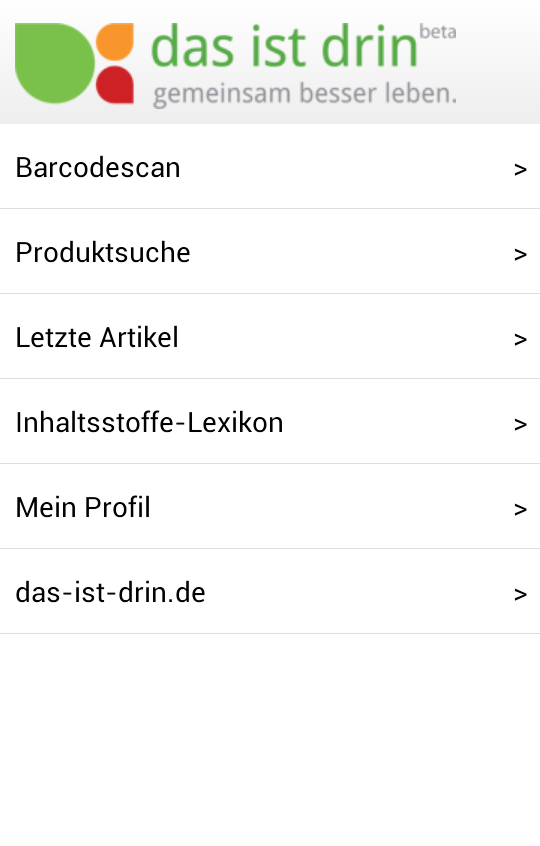
\includegraphics[width=\textwidth]{pics/did-1.png}}
		\caption{direkt nach Start der App}
		\label{img:did-1}
	\end{subfigure}
	~
	\begin{subfigure}[b]{0.45\textwidth}
		\frame{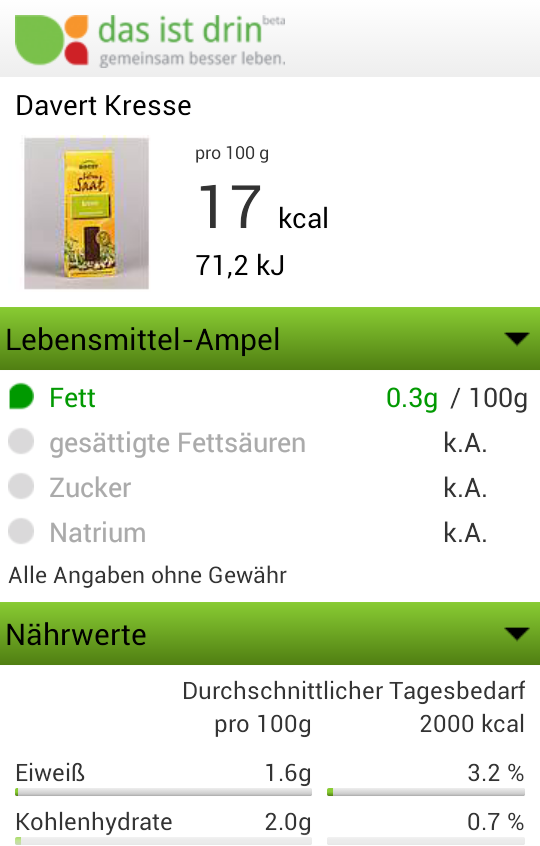
\includegraphics[width=\textwidth]{pics/did-2.png}}
		\caption{Ansicht nach Scan eines Barcodes mit ausgeklappten
		Reitern}
		\label{img:did-2}
	\end{subfigure}
	\caption[Mobile App von das-ist-drin für Android in Benutzung ]{Mobile App von
			das-ist-drin für Android in Benutzung \citeweb{did:app},
	aufgenommen am 05.05.2013}
	\label{img:did}
\end{figure}

Jedes Produkt enthält auf der Website -- sofern von den Nutzer*innen
angegeben -- Informationen zu Ernährungsweisen, darunter auch, ob das
Produkt vegan ist. Diese
Angaben fehlen jedoch in der mobilen Variante.

\section{EuLa-Armband}
\label{sec:eulaa}

In der Diplomarbeit von Anke Bretz wurde ein Prototyp, ein so
genanntes \ac{EuLaA}
entwickelt, der Menschen mit einer Lebensmittelallergie
bei der Auswahl von Produkten beim Einkaufen helfen soll \cite{bre07},
welcher in Abbildung~\ref{img:eula} dargestellt ist.\\
Bildausschnitt 1 zeigt den Prototyp nach dem Start, Bildausschnitt 2
deutet durch die grüne Umrandung nach Scan eines Produktes an, dass
dieses keine unverträglichen Inhaltsstoffe besitzt, Bildausschnitt 3
warnt mit einer gelben Umrandung und einem Warnschild, da eine
Lebensmittelunverträglichkeit vorliegt und fragt, ob es Alternativprodukte
vorschlagen soll und Bildausschnitt 4 signalisiert durch die rote
Umrandung und das Stoppschild ein nicht verträgliches Produkt und
zeigt direkt Alternativprodukte an.

\begin{figure}[ht]
	\centerline{
	  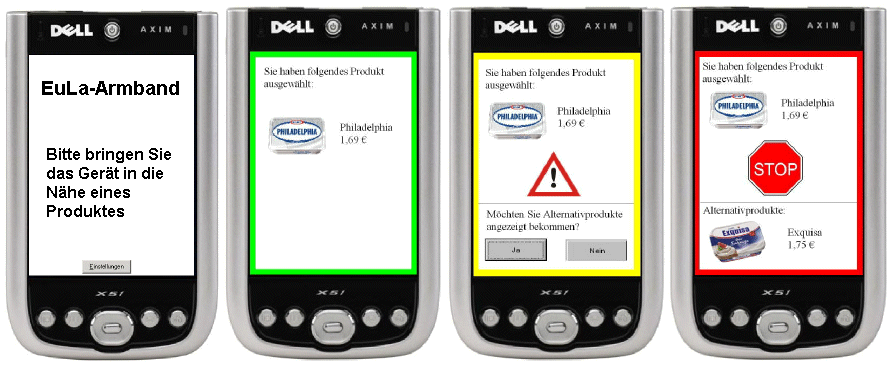
\includegraphics[scale=0.5]{pics/eula-2.png}
	}
	\caption[Beispielhafte Benutzung des EuLa-Armbands]{Beispielhafte Benutzung des EuLa-Armbands, modifiziertes Bild 
aus der Diplomarbeit \cite{bre07}}
	\label{img:eula}
\end{figure}

Als "`Armband"' wurde ein \ac{PDA} benutzt, welcher
statt der Identifikation eines Produktes mit Hilfe eines Barcodes
\ac{RFID} unterstützt.\\
Es gibt mehrere Datenbanken, je eine Patient*innen-,
Waren-, Geschäfte- und Warenwirtschaftsdatenbank. Letztere besteht
wiederum aus so vielen Datenbanken, wie Supermarktketten existieren.\\
Um \ac{EuLaA} länderübergreifend zu nutzen, wurden die
Produktdatenbanken exemplarisch mit englischen und deutschen Daten
bestückt.\\
Änderungen in den Datenbanken sind nicht durch eine*n Benutzer*in
möglich, sondern nur von den jeweiligen Institutionen
(z.\,B. ist die Patient*innendatenbank nur durch die behandelnden
Ärzte*Ärztinnen
editierbar, über die die Registrierung am System erfolgt,
die Warendatenbank nur durch unterschiedliche Firmen).\\
Ein Zugriff von außerhalb (bis auf den normalen Gebrauch) ist daher und
insbesondere durch hohe Sicherheitsstandards nicht möglich.

\section{\acs{MENSSANA}}
\label{sec:menssana}

Innerhalb des Projekts \ac{MENSSANA} werden Lösungen zur
Identifikation von Lebensmitteln gesucht, die Menschen mit Allergien
oder Unverträglichkeiten ohne Probleme zu sich nehmen können
\cite{ahsr07}.\\
Entwickelt wurde daher vom "`Centre de Recherche Public Henri Tudor"'
ein \ac{PAA} in Form einer \ac{App} und eine Website (WikiFood
\citeweb{wikifood}), die u.\,a.
Allergie-Informationen zu einem Produkt auch im Internet bereit
stellt \cite{arfhhm08}, \citeweb{menssana}.

\begin{figure}[ht]
	\centering
	\begin{subfigure}[b]{0.45\textwidth}
		\frame{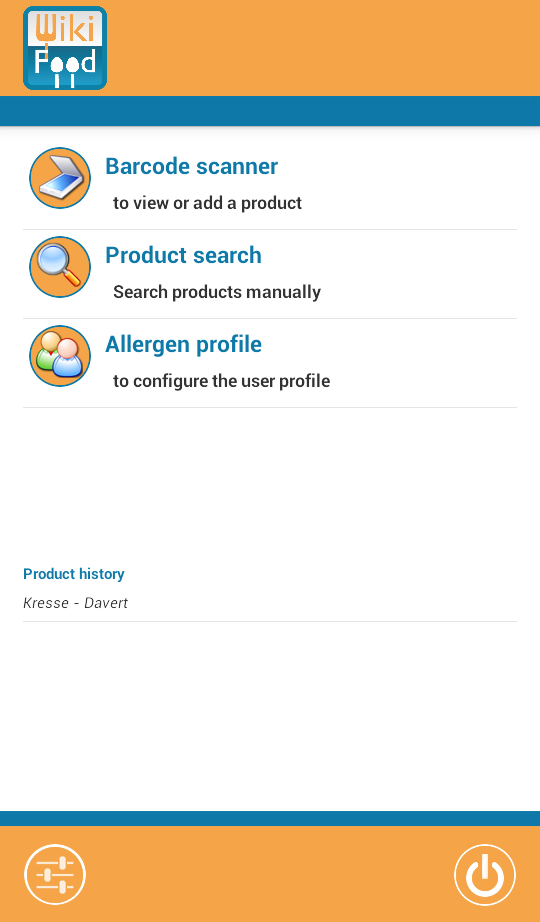
\includegraphics[width=\textwidth]{pics/wikifood-1.png}}
		\caption{zu Beginn}
		\label{img:wikifood-1}
	\end{subfigure}
	~
	\begin{subfigure}[b]{0.45\textwidth}
		\frame{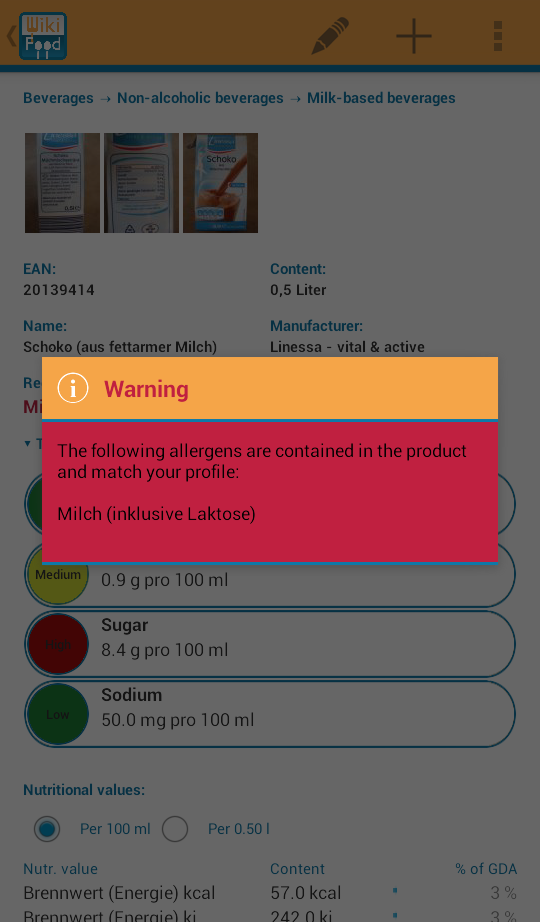
\includegraphics[width=\textwidth]{pics/wikifood-2.png}}
		\caption{Warnung bei einem Milchprodukt}
		\label{img:wikifood-2}
	\end{subfigure}
	\caption[Mobile App von WikiFood in Benutzung]{Mobile App von WikiFood in Benutzung
	\citeweb{wikifood:app}, aufgenommen am 05.05.2013}
	\label{img:wikifood}
\end{figure}

Der \ac{PAA}, welcher in Abbildung~\ref{img:wikifood} zu sehen ist, 
ist für das Android-Betriebssystem verfügbar
\citeweb{wikifood:app}.\\
Um die \ac{App} mit einem persönlichem Allergieprofil zu nutzen oder
neue Produkte in die Datenbank einzutragen oder zu ändern, ist
eine Anmeldung auf der deutsch-, englisch und französisch-sprachigen
Website erforderlich.\\
Wird nach Festlegung eines Allergieprofils ein Produkt gescannt, was
solch ein Allergen beinhaltet, wird eine Warnung mit einem Hinweis
eingeblendet, was in Abbildung~\ref{img:wikifood-2} dargestellt ist.\\
Die Website WikiFood wird u.\,a. mit Angaben direkt von Hersteller*innen, der
Datenbank "`ecoinform"' und von Benutzer*innen befüllt.\\
Zugriffe abseits vom normalen Gebrauch (bspw. per \ac{API}) sind aus
rechtlichen Gründen nicht möglich.

\clearpage
\section{Zusammenfassung}
\label{rel:zsf}

Nachfolgend wird in einer Tabelle dargestellt, wie sich die zu dieser Arbeit 
verwandten Arbeiten unterscheiden.
Dazu wird Bezug
genommen auf die einzelnen Kriterien, die zu Beginn des Kapitels
festgelegt wurden.\\
Die Kriterien sind:

\begin{itemize}
	\item \textbf{Veganität}: enthält der Dienst Informationen zur
			Veganität?
	\item \textbf{Plattformunabhängig}: gibt es das Angebot für
			mehr als ein Betriebssystem, also z.\,B. als Website und
			als mobile Applikation?
	\item \textbf{Lizenzfreiheit}: sind die Daten frei, d.\,h. ist z.\,B.
			ein \ac{API}-Zugriff oder ein kompletter Speicherauszug
			der Datenbank möglich?
	\item \textbf{Zugang}: sind die Informationen zu den Produkten
			auch ohne Anmeldung erhältlich?
	\item \textbf{Ursprung}: stammen die Daten von der
			Internetcommunity, also den Nutzer*innen?
	\item \textbf{Lokalisierung}: ist der Dienst lokalisiert, d.\,h. werden auch andere
			Sprachen als Deutsch unterstützt?
\end{itemize}

\begin{table}[htb]
\begin{adjustwidth}{-1in}{-1in}% adjust the L and R margins by 1 inch
\centering
\rowcolors{2}{gray!25}{white}
\begin{tabular}{rccccc}
	 &
	\rot{\textbf{barcoo}} &
	\rot{\textbf{das-ist-drin}} &
	\rot{\textbf{EuLa-Armband}} &
	\rot{\textbf{MENSSANA}}\\
	\hline

	\textbf{Veganität} &
	(\cmark) &
	(\cmark) &
	\xmark &
	(\cmark)\\
	
	\textbf{Plattformunabhängig} &
	\cmark &
	\cmark &
	\xmark &
	\cmark\\

	\textbf{Lizenzfreiheit} &
	\xmark &
	\xmark &
	\xmark &
	\xmark\\
	
	\textbf{Zugang} &
	\cmark &
	\cmark &
	\xmark &
	\cmark\\
	
	\textbf{Nutzer*innenbasiert} &
	\xmark &
	\cmark &
	\xmark &
	(\cmark)\\

	\textbf{Lokalisierung} &
	\xmark &
	\xmark &
	\cmark &
	\cmark\\

\end{tabular}
\caption{Gegenüberstellung der verwandten
Arbeiten anhand 
verschiedener Kriterien}
\end{adjustwidth}
\end{table}
\medskip % adds some space after the table

Während \ac{EuLaA} keine veganismusrelevanten Daten beinhaltet, sind bei
barcoo, \ac{DID} und \ac{MENSSANA} vegane Daten zu finden
(symbolisiert durch das \cmark\ in Klammern).
Allerdings liegen diese nicht bei allen Produkten vor und beinhalten keine 
genauen Quellen wie
Produktanfragen (siehe Abschnitt~\ref{sec:inquiry}), während dies in dieser
Arbeit der Fall sein soll.\\
Alle Dienste außer \ac{EuLaA} sind plattformunabhängig, d.\,h.
bieten zusätzlich zu einer Website mindestens eine mobile Anwendung
an, was die Nutzung unterwegs erleichtert. Dies soll auch in dieser
Arbeit der Fall sein.\\
Während alle anderen
Dienste die Produktdaten nicht offenlegen oder nur mit Einschränkungen
erreichbar machen, soll dies hier nicht der Fall sein.\\
Der Zugang zu den Produktinformationen, d.\,h. die Ansicht ist bei
allen Diensten außer bei \ac{EuLaA} ohne Anmeldung
gewährleistet. Der freie Zugang ist auch in dieser Arbeit vorgesehen.\\
Die Daten der einzelnen Dienste stammen bei barcoo und 
\ac{EuLaA}
nicht von den Nutzer*innen, bei \ac{MENSSANA} teilweise, während
\ac{DID} nach dem Wikiprinzip funktioniert und die Daten von den
Nutzer*innen verwaltet werden. Das Wikiprinzip soll auch in diesem Werk zu einer 
umfangreichen Datenbank führen.\\
\ac{EuLaA} ist international verfügbar, da es für jedes Land eine
eigene Datenbank gibt, MENSSANA ist dreisprachig verfügbar und barcoo 
sowie \ac{DID} liegen jeweils in einer deutschen Version vor.
Die vorliegende Arbeit soll durch Sprachdateien und Zutatensynonyme international
gemacht werden können.

Die Besonderheit dieser Arbeit im Hinblick auf die verwandten Arbeiten soll die 
Belegung der veganen Daten mit Quellen sein. Dies soll für vegan lebende Menschen in 
Verbindung mit der Plattformunabhängig von Vorteil sein, da diese überall 
leicht 
nachschauen können, ob ein Produkt vegan ist oder nicht. Insbesondere soll 
diese Arbeit dazu genutzt werden, eine Datenbank mit lizenzfreien Daten 
aufzubauen, die anschließend für andere Zwecke gebraucht werden kann. Z.\,B. 
um herauszufinden, ob 
ein Produkt tierversuchsfrei, roh oder fair ist oder um einen schon vorhandenen 
Dienst mit diesen Daten zu erweitern.